
%(BEGIN_QUESTION)
% Copyright 2005, Tony R. Kuphaldt, released under the Creative Commons Attribution License (v 1.0)
% This means you may do almost anything with this work of mine, so long as you give me proper credit

Determine what the output response will be to a positive-ramping voltage applied at the input of these (ideal) circuits:

$$\includegraphics[width=15.5cm]{i01571x01.eps}$$

\vskip 20pt \vbox{\hrule \hbox{\strut \vrule{} {\bf Suggestions for Socratic discussion} \vrule} \hrule}

\begin{itemize}
\item{} Identify practical applications in industry for circuits such as these.
\item{} Identify what would have to be different about the input signal to each circuit in order to generate a {\it negative} output voltage.
\item{} Explain how each of these circuits would respond to a sinusoidal input signal of constant frequency.
\item{} Explain how each of these circuits would respond to a sinusoidal input signal of increasing frequency.
\item{} Explain what would happen if the output of the integrator were connected to the input of the differentiator, and then a signal was input to the integrator.  What kind of signal would come out of the differentiator?
\item{} Explain what would happen if the output of the differentiator were connected to the input of the integrator, and then a signal was input to the differentiator.  What kind of signal would come out of the integrator?
\end{itemize}

\underbar{file i01571}
%(END_QUESTION)





%(BEGIN_ANSWER)

$$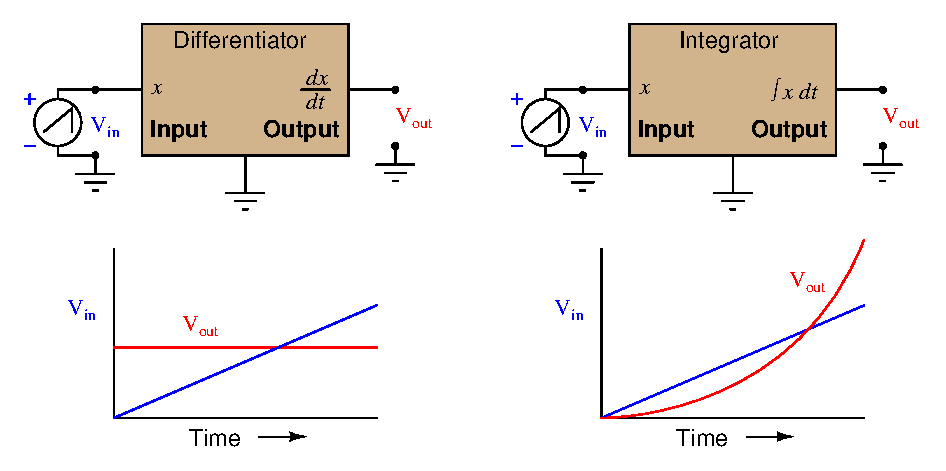
\includegraphics[width=15.5cm]{i01571x02.eps}$$

%(END_ANSWER)





%(BEGIN_NOTES)

Ask your students to frame their answers in a practical context, such as speed and distance for a moving object (where speed is the time-derivative of distance and distance is the time-integral of speed).

%INDEX% Electronics review: differentiator circuit response
%INDEX% Electronics review: integrator circuit response

%(END_NOTES)


